%! Author = cspiller
%! Date = 17/11/2022

\thispagestyle{plain}
\newpage
\section{Project Plan}\label{sec:project-plan}

\normalsize

\subsection{Plan Preparation and Communication}\label{subsec:plan-preparation-and-communication}

To develop an effective plan for the project, the key deliverables for the project\footnote{As outlined in~\ref{subsec:project-objectives}} were analysed and roughly estimated based upon the perceived complexity of producing that deliverable.
Each deliverable was given a broad estimate of the time this would take in proportion to that complexity, with more complex tasks, and tasks that were prone to delay, given more breathing room in the time allocated to them.
These estimates were then mapped to the overall timescale of the project, and set dates were then applied to the completion of these deliverables in relation to the key milestones of the project, such as submission deadlines.
Subsequently, the broader deliverables were then broken down into subtasks and milestones to provide a more granular view of the project plan.
Text-based artefacts were given dates by which certain chapters needed to be completed, and development tasks were given dates by which certain parts of the application should be built and deployed by.
These subtasks helped to keep track of the project’s progress.

This project makes use of the ClickUp\footnote{\citep{clickup}} software to perform project management functions and to organize this author’s workflow.
This software has been chosen over other pieces of software in the education\footnote{\citep{education_software}} and project management\footnote{\citep{pm_software}} space on the basis of cost and ease-of-use, as well as its ability to synchronize across different platforms.
In addition, the platform was also used to communicate the project's progress with the project supervisor who is able to see the project plan and its progress over time through the updating of subtask statuses.

Prioritizing communication with the supervisor was integral to the success of the project because of the accountability and oversight it provided to this author.
Having a platform such as ClickUp drastically reduced the likelihood of error in communication and time management.
Additionally, a meeting with the project supervisor was scheduled every two weeks in order to identify and rememdy issues with the project's execution.

\subsection{Timeline}\label{subsec:timeline}

The below series of figures (\ref{fig:timeline1},~\ref{fig:timeline2},~\ref{fig:timeline3}) detail the tasks, subtasks, and the planned timeframes for completion.
Timeframes were adjusted in accordance with the perceived complexity of each task following enlightenment from the literature review and market research.
Dependencies for each task were also calculated and can be seen as arrow representation in the timeline figures.

\begin{figure}[!htb]
    \minipage{\textwidth}
    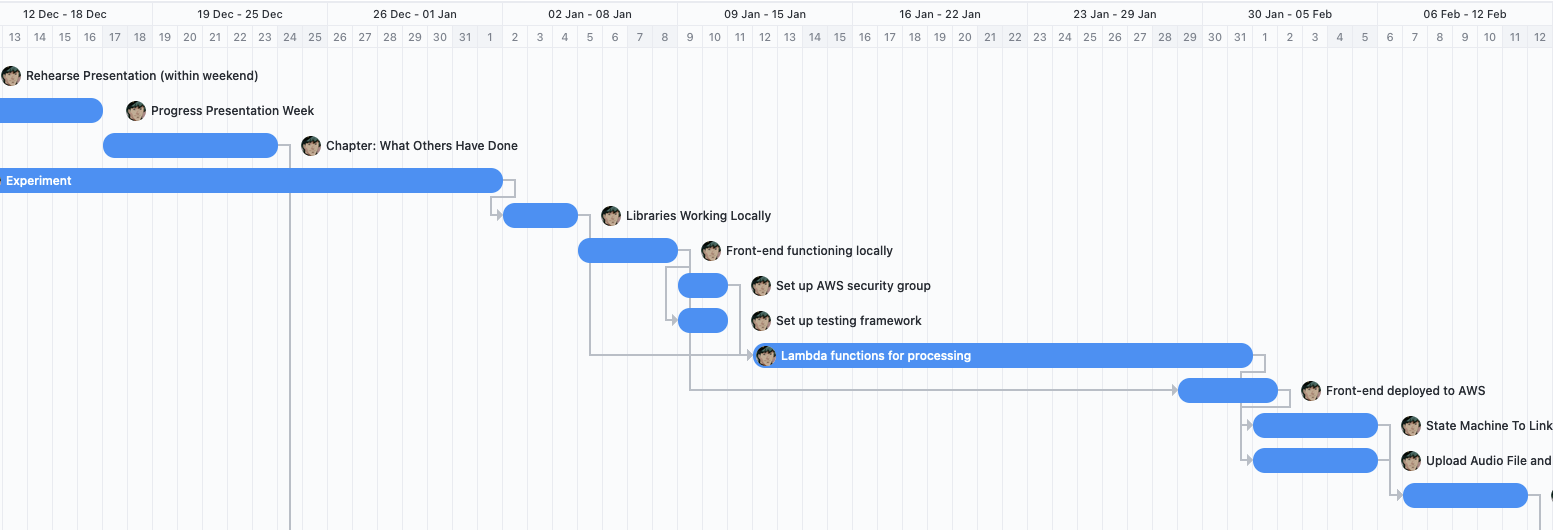
\includegraphics[width=\linewidth]{timeline1}
    \caption{Timeline: $Dec~12th~\rightarrow~Feb~12th$}\label{fig:timeline1}
    \endminipage\hfill
    \minipage{\textwidth}
    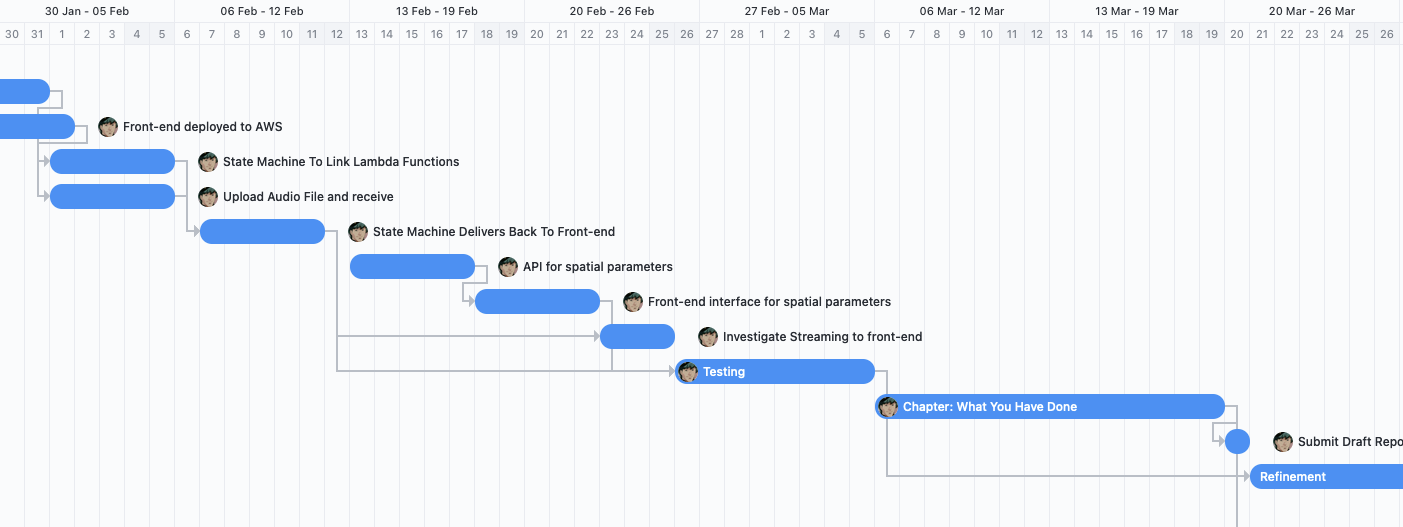
\includegraphics[width=\linewidth]{timeline2}
    \caption{Timeline: $Jan~30th~\rightarrow~Mar~26th$}\label{fig:timeline2}
    \endminipage\hfill
    \minipage{\textwidth}
    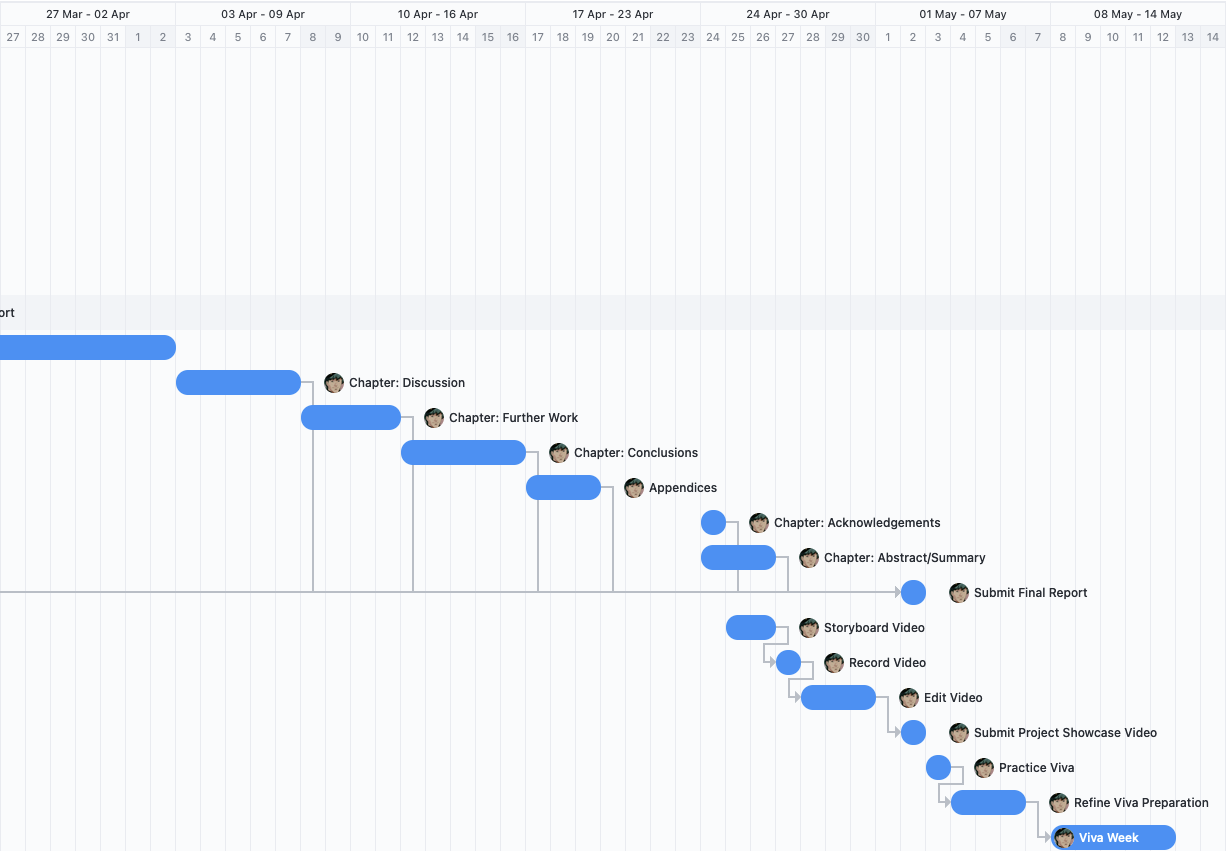
\includegraphics[width=\linewidth]{timeline3}
    \caption{Timeline: $Mar~27th~\rightarrow~May~14th$}\label{fig:timeline3}
    \endminipage
\end{figure}

\subsection{Resources}\label{subsec:resources}

This project intended to use minimal resources in its development.
As outlined in~\ref{sec:literature-review}, one of the many advantages of cloud computing is its flexibility and ease of resource management.
Given that the application would be hosted entirely in cloud environments, there would be no hardware costs associated with the project.
The costs that do apply will relate to the use of the~\gls{aws} platform.
These costs needed careful management, as explained in~\ref{subsec:business-risks}.

Other resources utilized included:

\begin{enumerate}
    \item Queen Mary library resources
    \item The project supervisor
    \item Knowledge sharing from colleagues at~\gls{sie}
    \item JetBrains’~\gls{ide} Suite
    \item Open-source audio-processing libraries.
    \item Online articles and tutorials
\end{enumerate}

\subsection{Methodology}\label{subsec:methodology}

\citet{murray-pm} notes that the \textquote{traditional} manner of software development follows a linear path from requirements, to design, to execution, to testing, and so on.
This method often results in inflexibility when it comes to software project execution.
This is because of its dependence on the full set of requirements being gathered before the development process begins.
Any issues with the requirements (incompleteness, inaccuracy) using this method are typically only found at the end of the process, instead of along the way through a cycle of development and feedback\footnote{\citep{murray-pm}}.
This project is of relatively small scope, and the number of shareholders are small on account of its proof-of-concept status.
As such, it serves to incorporate some, but not all, aspects of the `Agile'\footnote{\citep{beck2001agile}} development methodology into the process:

\begin{quotation}
    An Agile project starts with only the most high-level requirements.
    Sometimes these are referred to as “user stories.”
    Such a requirement might sound like, “A user will be able to buy a subscription to our product on a new e-commerce website.”
    There are no designs, no specifications.\footnote{\citep{murray-pm}}
\end{quotation}

While this project will not go so far as to remove the need for a design or specification altogether, the foundation for the project’s execution will rest on high-level user stories and identified functional requirements.
In addition, the project will require frequent testing as development progresses.
The intention, therefore, is to endeavour to implement a~\gls{cicd} pipeline to ensure any updates to the prototype can be tested and deployed in an online environment as it is being developed.
